%Version 2.1 April 2023
% See section 11 of the User Manual for version history
%
%%%%%%%%%%%%%%%%%%%%%%%%%%%%%%%%%%%%%%%%%%%%%%%%%%%%%%%%%%%%%%%%%%%%%%
%%                                                                 %%
%% Please do not use \input{...} to include other tex files.       %%
%% Submit your LaTeX manuscript as one .tex document.              %%
%%                                                                 %%
%% All additional figures and files should be attached             %%
%% separately and not embedded in the \TeX\ document itself.       %%
%%                                                                 %%
%%%%%%%%%%%%%%%%%%%%%%%%%%%%%%%%%%%%%%%%%%%%%%%%%%%%%%%%%%%%%%%%%%%%%

\documentclass[sn-nature,referee,pdflatex]{sn-jnl}

%%%% Standard Packages
%%<additional latex packages if required can be included here>

\usepackage{graphicx}%
\usepackage{multirow}%
\usepackage{amsmath,amssymb,amsfonts}%
\usepackage{amsthm}%
\usepackage{mathrsfs}%
\usepackage[title]{appendix}%
\usepackage{xcolor}%
\usepackage{textcomp}%
\usepackage{manyfoot}%
\usepackage{booktabs}%
\usepackage{algorithm}%
\usepackage{algorithmicx}%
\usepackage{algpseudocode}%
\usepackage{listings}%
%%%%

%%%%%=============================================================================%%%%
%%%%  Remarks: This template is provided to aid authors with the preparation
%%%%  of original research articles intended for submission to journals published
%%%%  by Springer Nature. The guidance has been prepared in partnership with
%%%%  production teams to conform to Springer Nature technical requirements.
%%%%  Editorial and presentation requirements differ among journal portfolios and
%%%%  research disciplines. You may find sections in this template are irrelevant
%%%%  to your work and are empowered to omit any such section if allowed by the
%%%%  journal you intend to submit to. The submission guidelines and policies
%%%%  of the journal take precedence. A detailed User Manual is available in the
%%%%  template package for technical guidance.
%%%%%=============================================================================%%%%

\usepackage{comment}
\usepackage{anyfontsize}
\usepackage[style=default]{caption}
\usepackage{float}
\usepackage{placeins}
\usepackage{booktabs}
\usepackage{longtable}
\usepackage{array}
\usepackage{multirow}
\usepackage{wrapfig}
\usepackage{float}
\usepackage{colortbl}
\usepackage{pdflscape}
\usepackage{tabu}
\usepackage{threeparttable}
\usepackage{threeparttablex}
\usepackage[normalem]{ulem}
\usepackage{makecell}
\usepackage{xcolor}


\raggedbottom




% tightlist command for lists without linebreak
\providecommand{\tightlist}{%
  \setlength{\itemsep}{0pt}\setlength{\parskip}{0pt}}





\begin{document}


\title[MAP-reduction-meta]{Meaningfully reducing consumption of meat and
animal products is an unsolved problem: \newline A meta-analysis}

%%=============================================================%%
%% Prefix	-> \pfx{Dr}
%% GivenName	-> \fnm{Joergen W.}
%% Particle	-> \spfx{van der} -> surname prefix
%% FamilyName	-> \sur{Ploeg}
%% Suffix	-> \sfx{IV}
%% NatureName	-> \tanm{Poet Laureate} -> Title after name
%% Degrees	-> \dgr{MSc, PhD}
%% \author*[1,2]{\pfx{Dr} \fnm{Joergen W.} \spfx{van der} \sur{Ploeg} \sfx{IV} \tanm{Poet Laureate}
%%                 \dgr{MSc, PhD}}\email{iauthor@gmail.com}
%%=============================================================%%

\author*[1]{\fnm{Seth
Ariel} \sur{Green} }\email{\href{mailto:setgree@stanford.edu}{\nolinkurl{setgree@stanford.edu}}}

\author[1]{\fnm{Maya B.} \sur{Mathur} }

\author[2]{\fnm{Benny} \sur{Smith} }



  \affil[1]{\orgdiv{Quantitative Sciences Unit, Department of
Medicine}, \orgname{Stanford University}}
  \affil[2]{\orgname{Allied Scholars for Animal Protection}}

\abstract{Which interventions produce the largest and most enduring
reductions in consumption of meat and animal products (MAP)? We address
this question with a theoretical review and meta-analysis of randomized
controlled trials that measured MAP consumption at least one day after
intervention. We meta-analyze 35 papers comprising 41 studies, 112
interventions, and approximately 87,000 subjects. We find that these
papers employ four major strategies to change behavior: choice
architecture, persuasion, psychology, and a combination of persuasion
and psychology. The pooled effect of all 112 interventions on MAP
consumption is quite small (standardized mean difference (SMD) = 0.07
(95\% CI: {[}0.02, 0.12{]}), indicating an unsolved problem.
Interventions aiming to reduce only consumption of red and processed
meat were more effective (SMD = 0.25; 95\% CI: {[}0.11, 0.38{]}), but it
remains unclear whether such interventions increase consumption of other
forms of MAP. but it remains unclear whether such interventions also
decrease consumption of other forms of MAP. We conclude that while
existing approaches do not provide a proven remedy to MAP consumption,
designs and measurement strategies have generally been improving over
time, and many promising interventions await rigorous evaluation.}

\keywords{meta-analysis, meat, plant-based, randomized controlled
trial, climate change, sustainability}



\maketitle

\section{Introduction}\label{sec1}

Global consumption of meat and animal products (MAP) is increasing
\citep{godfray2018} and is expected to continue doing so
\citep{whitton2021}. Abating this trend is vital to reducing chronic
diseases caused by excessive MAP consumption and the risk of zoonotic
pandemics \citep{willett2019, landry2023, hafez2020}, mitigating
environmental degradation and climate change
\citep{poore2018, koneswaran2008, greger2010}, and improving animal
welfare \citep{kuruc2023, scherer2019}. However, eating MAP is widely
regarded as normal, ethical, and necessary
\citep{piazza2022, milford2019}.

There is a vast and diverse literature investigating potential means to
reduce MAP consumption. Example approaches include providing free access
to meat substitutes \citep{katare2023}, changing the price
\citep{horgen2002} or perceptions \citep{kunst2016} of meat, and
attempting to persuade people to change their diets
\citep{bianchi2018conscious}. Some interventions are associated with
large impacts \citep{lentz2020, boronowsky2022, reinders2017}, and prior
reviews have concluded that some frequently studied approaches, such as
using persuasive messaging that appeals to animal welfare
\citep{mathur2021meta}, may be consistently effective. A particularly
high-profile strand of this literature employs choice architecture,
i.e.~altering the contexts in which MAP is selected
\citep{bianchi2018restructuring}, for instance by changing menu layouts
\citep{bacon2018, gravert2021}, placing vegetarian items more
prominently in dining halls \citep{ginn2024}, or making plant-based
options the default at catered meals \citep{hansen2021}. Choice
architecture could be a cheap, effective way of altering dietary
behavior \citep{colgan2024}, and governments, universities, and other
institutions are increasingly implementing these approaches in such
settings as dining halls \citep{pollicino2024} and hospital cafeterias
\citep{morgenstern2024}.

However, recurring design and measurement limitations compromise the
literature on MAP reduction. Many interventions are either not
randomized \citep{garnett2020} or underpowered \citep{delichatsios2001}.
Measured outcomes are often imperfect proxies of MAP consumption, such
as attitudes, intentions, and hypothetical choices
\citep{raghoebar2020, vermeer2010}, yet behaviors often do not track
with these psychological processes
\citep{mathur2021effectiveness, porat2024} and reported preferences
\citep{hensher2010}. Additionally, many studies with comparatively large
effects specifically aim to reduce consumption of red and processed meat
(RPM). However, because these studies exclusively measure changes in
RPM, it is unknown whether they induce substitution to other forms of
MAP, such as chicken or fish \citep{grummon2023}. Thus, treating RPM
consumption as a proxy of net MAP reduction, as prior reviews have done
\citep{bianchi2018conscious, chang2023, kwasny2022}, may cause bias.
Finally, many studies measure only immediate rather than long-term
effects \citep{hansen2021, griesoph2021}. This is of special concern if
subjects who are encouraged to have a single vegetarian meal later
compensate by consuming more MAP, which would make an immediate outcome
measurement a biased estimate of overall effects. Such compensatory
effects are common in dietary studies
\citep{yeomans2001, robinson2013, lowe2007}.

In the past few years, a new wave of MAP reduction research has made
commendable methodological advances in design, measurement validity, and
statistical power. Historically, in some scientific fields, strong
effects detected in early studies with methodological limitations were
ultimately overturned by more rigorous follow-ups
\citep{wykes2008, paluck2019, scheel2021}. Does this phenomenon hold in
the MAP reduction literature as well?

To address this question, we conducted a meta-analysis of randomized
controlled trials (RCTs) that aim to reduce MAP consumption and that
meet basic methodological standards
\citep{andersson2021, kanchanachitra2020, abrahamse2007, acharya2004, banerjee2019, bianchi2022, bochmann2017, bschaden2020, carfora2023, cooney2014, cooney2016, feltz2022, haile2021, hatami2018, hennessy2016, jalil2023, mathur2021effectiveness, merrill2009, norris2014, peacock2017, polanco2022, sparkman2021, weingarten2022, piester2020, aberman2018, aldoh2023, allen2002, camp2019, coker2022, sparkman2020, berndsen2005, bertolaso2015, fehrenbach2015, mattson2020, shreedhar2021}.
Specifically, we restricted eligibility to RCTs that measured
consumption outcomes at least a single day after treatment was first
administered and that had at least 25 subjects in both treatment and
control (or, for cluster-assigned studies, at least ten clusters in
total).

Studies in our meta-analysis pursued one of four theoretical approaches:
choice architecture, psychological appeals (typically manipulations of
perceived norms around eating meat), explicit persuasion (centered
around animal welfare, the environment, and/or health), or a combination
of psychological and persuasion messages. Interventions varied in
delivery method, for example, documentary films
\citep{mathur2021effectiveness}, leaflets \citep{peacock2017},
university lectures \citep{jalil2023}, op-eds \citep{haile2021}, and
changes to menus in cafeterias \citep{andersson2021} and restaurants
\citep{coker2022, sparkman2021}. We estimated overall effect sizes as
well as effect sizes associated with different theoretical approaches
and delivery mechanisms. Although we find some heterogeneity across
theories and mechanisms, we find consistently smaller effects on MAP
consumption than previous reviews that placed fewer (if any)
restrictions on studies' outcomes and methodological rigor
\citep{bianchi2018restructuring, byerly2018, chang2023, harguess2020, kwasny2022, mathur2021meta, meier2022}.
When we included studies whose methodology fell short of our inclusion
criteria
\citep{alblas2023, beresford2006, betterfoodfoundation2023, celis2017, dannenberg2023, delichatsios2001eatsmart, epperson2021, frie2022, garnett2020, griesoph2021, hansen2021, johansen2009, kaiser2020, lentz2019, loy2016, matthews2019, piazza2022, reinders2017, sparkman2017},
this considerably increased the pooled estimate. In addition, studies
that only aimed to reduce RPM consumption
\citep{anderson2017, carfora2017correlational, carfora2017randomised, carfora2019, carfora2019informational, delichatsios2001talking, dijkstra2022, emmons2005cancer, emmons2005project, jaacks2014, james2015, lee2018, lindstrom2015, perino2022, schatzkin2000, sorensen2005, wolstenholme2020},
reported consistently stronger effects on behavior than studies aimed at
reducing net MAP consumption. Overall, in contrast to previous reviews,
we conclude that meaningfully reducing net MAP consumption is an
unsolved problem, although many promising approaches still await
rigorous evaluation.

\section{Results}\label{sec2}

\subsection{Results across all studies}\label{sec2.1}

Our meta-analysis included 35 papers comprising 41 studies and 112
separate point estimates. Each point estimate corresponded to a distinct
intervention. The total sample size was approximately 87,000 subjects.

Because methodological quality is rapidly improving in this literature,
the majority of eligible papers (18 of 35) were published from 2020
onwards, although the earliest was published in 2002 \citep{allen2002}.
Among studies where treatment was assigned to individuals rather than to
clusters (e.g., school classes), the median analyzed sample size per
study was 132 subjects (25\textsuperscript{th}--75\textsuperscript{th}
percentiles: 109, 208).

We found that studies' theoretical approaches could be grouped into four
categories. \textbf{Choice architecture} studies
\citep{andersson2021, kanchanachitra2020} (n = 2 studies with 3
estimates) manipulate aspects of physical environments to reduce MAP
consumption, such as by placing the vegetarian option at eye level on a
cafeteria's billboard menu \citep{andersson2021}. \textbf{Persuasion}
studies
\citep{kanchanachitra2020, aberman2018, abrahamse2007, acharya2004, banerjee2019, bianchi2022, bochmann2017, bschaden2020, carfora2023, hennessy2016, piester2020, cooney2014, cooney2016, feltz2022, haile2021, hatami2018, jalil2023, mathur2021effectiveness, merrill2009, norris2014, peacock2017, polanco2022, sparkman2021, weingarten2022}
(n = 25 studies with 77 estimates) focus on health, environmental
(usually climate change), and animal welfare reasons to reduce MAP
consumption. Such messages are often delivered through printed
materials, such as leaflets \citep{haile2021, polanco2022}, booklets
\citep{bianchi2022} articles and op-eds \citep{sparkman2021, feltz2022},
and videos \citep{sparkman2021, cooney2016, mathur2021effectiveness}.
Less common delivery methods included in-person dietary consultations
\citep{merrill2009}, emails \citep{banerjee2019}, and text messages
\citep{carfora2023}. \textbf{Psychology} studies
\citep{aldoh2023, allen2002, camp2019, coker2022, piester2020, sparkman2020}
(n = 9 studies with 12 estimates) manipulate the interpersonal,
cognitive, or affective factors associated with eating MAP. The most
common psychological intervention is centered on social norms seeking to
alter the perceived popularity of non-MAP dishes
\citep{sparkman2020, sparkman2021}. In one study, a restaurant put up
signs stating that ``{[}m{]}ore and more {[}retail store name{]}
customers are choosing our veggie options'' \citep{coker2022}. In
another, a university cafeteria put up signs stating that ``{[}i{]}n a
taste test we did at the {[}name of cafe{]}, 95\% of people said that
the veggie burger tasted good or very good!'' \citep{piester2020}. One
study told participants that people who ate meat are more likely to
endorse social hierarchy and embrace human dominance over nature
\citep{allen2002}. Other psychological interventions include response
inhibition training, where subjects are trained to avoid responding
impulsively to stimuli such as unhealthy food \citep{camp2019}, and
implementation intentions, where participants list potential challenges
and solutions to changing their own behavior
\citep{aberman2018, shreedhar2021}. Finally, some studies combine
\textbf{persuasion} approaches with \textbf{psychological} appeals to
reduce MAP consumption
\citep{aberman2018, berndsen2005, bertolaso2015, carfora2023, fehrenbach2015, hennessy2016, mathur2021effectiveness, mattson2020, piester2020, shreedhar2021}
(n = 11 studies with 20 estimates). These studies typically combine a
persuasive message with a norms-based appeal
\citep{piester2020, mattson2020} or an opportunity to pledge to reduce
one's MAP consumption \citep{mathur2021effectiveness, shreedhar2021}.

\begin{table}[!ht]
\centering
\caption{\label{tab:table_one}Meta-analytic Results Overall and by Theoretical Approach}
\centering
\begin{tabular}[t]{llllll}
\toprule
Approach & N (Studies) & N (Estimates) & SMD & 95\% CIs & $p$ val\\
\midrule
Overall & 41 & 112 & 0.07 & {}[0.02, 0.12] & .007\\
\addlinespace[0.5em]
\multicolumn{6}{l}{\textbf{Theory}}\\
\hspace{1em}Choice Architecture & 2 & 3 & 0.21 & {}[-0.99, 1.42] & .267\\
\hspace{1em}Psychology & 19 & 32 & 0.10 & {}[0, 0.2] & .054\\
\hspace{1em}Persuasion & 25 & 77 & 0.07 & {}[0.01, 0.13] & .023\\
\hspace{1em}Persuasion \& Psychology & 11 & 20 & 0.11 & {}[-0.06, 0.28] & .189\\
\addlinespace[0.5em]
\multicolumn{6}{l}{\textbf{Type of Persuasion}}\\
\hspace{1em}Animal Welfare & 16 & 65 & 0.03 & {}[-0.02, 0.07] & .189\\
\hspace{1em}Environment & 15 & 28 & 0.09 & {}[-0.03, 0.2] & .115\\
\hspace{1em}Health & 18 & 30 & 0.08 & {}[-0.01, 0.17] & .068\\
\bottomrule
\multicolumn{6}{l}{\textsuperscript{} Studies could occupy multiple categories for both theory and type of persuasion. Note that the}\\
\multicolumn{6}{l}{Ns for Types of Persuasion draws from both Persuasion and Persuasion and Psychology studies,}\\
\multicolumn{6}{l}{and that some studies with multiple interventions are represented in multiple theoretical}\\
\multicolumn{6}{l}{categories.}\\
\end{tabular}
\end{table}

In our dataset, the pooled effect of all interventions is standardized
mean difference (SMD) = 0.07 (95\% CI: {[}0.02, 0.12{]}), p = .007, with
some heterogeneity (standard deviation of population effects \(\tau\) =
0.082). Given the pooled effect size and the estimated heterogeneity, we
estimate that 26\% of true effects are above SMD = 0.1, and just 8\% are
above SMD = 0.2 \citep{mathur2019, mathur2020robust}.

\subsection{Subset and moderator analyses}\label{Sec2.2}

Stratifying by theoretical approach, pooled estimates were similar
across psychology, persuasion, and persuasion and psychology (SMDs from
0.07 to 0.11; Table 1). Estimates may have been somewhat larger among
the choice architecture studies (SMD = 0.21), but the sample size was
much smaller (3 estimates). Within studies with a persuasion component,
pooled estimates are similar for environmental appeals (SMD = 0.09, 15
studies with 28 estimates), and health appeals (SMD = 0.08, 18 studies
with 30 estimates), but are smaller for appeals to animal welfare (SMD =
0.03, 16 studies with 65 estimates). We did not conduct meta-regression
for theoretical approach or type of persuasion because studies with
multiple interventions could occupy multiple categories, and many
persuasion interventions combined multiple types of message,
e.g.~presenting students with both environmental and health reasons to
reduce MAP consumption \citep{jalil2023}.

\begin{figure}[H]

{\centering \includegraphics[width=120mm,]{./figures/forest_plot-1} 

}

\caption{Forest plot of all meta-analyzed studies. For papers contributing multiple point estimates, the plotted point corresponds to a fixed effects meta-analysis for each paper for visual clarity. Papers employing multiple theoretical approaches are represented once per theory. Point size is inversely proportional to variance. Points are sorted within theory by estimate size. The vertical black line demarcates an effect size of zero, and the dotted line is the observed overall effect.}\label{fig:forest_plot}
\end{figure}

Table 2 displays subset analyses and average differences in effect size
by study population, region, era of publication, and delivery method.

\begin{table}[!ht]

\caption{\label{tab:table_S1}Moderator Analysis Results}
\begin{tabular}[t]{lllll>{\raggedright\arraybackslash}p{2 cm}>{\raggedright\arraybackslash}p{2 cm}}
\toprule
Study Characteristic & N (Studies) & N (Estimates) & SMD & 95\% CIs & Subset $p$ value & Moderator $p$ value\\
\midrule
\addlinespace[0.3em]
\multicolumn{7}{l}{\textbf{Outcome}}\\
\hspace{1em}Meat and animal products & 41 & 112 & 0.07 & {}[0.02, 0.12] & .007 & \textbf{ref}\\
\hspace{1em}Red and processed meat & 17 & 25 & 0.25 & {}[0.11, 0.38] & .002 & .046\\
\addlinespace[0.3em]
\multicolumn{7}{l}{\textbf{Population}}\\
\hspace{1em}University students/staff & 18 & 38 & 0.07 & {}[-0.03, 0.16] & .139 & \textbf{ref}\\
\hspace{1em}All ages & 3 & 6 & 0.04 & {}[-0.16, 0.25] & .361 & .733\\
\hspace{1em}Adults & 17 & 61 & 0.09 & {}[0.01, 0.18] & .034 & .714\\
\hspace{1em}Adolescents & 3 & 6 & 0.02 & {}[-0.4, 0.44] & .806 & .686\\
\addlinespace[0.3em]
\multicolumn{7}{l}{\textbf{Region}}\\
\hspace{1em}North America & 23 & 74 & 0.04 & {}[-0.01, 0.08] & .142 & \textbf{ref}\\
\hspace{1em}Europe & 14 & 28 & 0.14 & {}[0.02, 0.27] & .029 & .156\\
\hspace{1em}Multi-region & 1 & 4 & 0.21 & {}[0.21, 0.21] & 0 & .000\\
\hspace{1em}Asia + Australia & 2 & 5 & 0.13 & {}[-0.17, 0.43] & .116 & .220\\
\addlinespace[0.3em]
\multicolumn{7}{l}{\textbf{Publication Decade}}\\
\hspace{1em}2000s & 6 & 8 & 0.16 & {}[-0.12, 0.43] & .199 & \textbf{ref}\\
\hspace{1em}2010s & 12 & 31 & 0.07 & {}[-0.03, 0.17] & .13 & .464\\
\hspace{1em}2020s & 23 & 73 & 0.05 & {}[-0.01, 0.11] & .074 & .369\\
\addlinespace[0.3em]
\multicolumn{7}{l}{\textbf{Method of Delivery}}\\
\hspace{1em}Educational materials & 15 & 59 & 0.01 & {}[-0.04, 0.07] & .566 & \textbf{ref}\\
\hspace{1em}Online & 8 & 22 & 0.16 & {}[-0.02, 0.34] & .067 & .170\\
\hspace{1em}Dietary consultation & 2 & 2 & 0.40 & {}[-3.36, 4.15] & .409 & .441\\
\hspace{1em}In-cafeteria & 8 & 13 & 0.10 & {}[-0.04, 0.25] & .101 & .123\\
\hspace{1em}Video & 10 & 16 & 0.01 & {}[-0.05, 0.07] & .485 & .533\\
\bottomrule
\multicolumn{7}{l}{\textsuperscript{} Moderation analyses by differences in outcomes, population, region, decade of publication, and delivery method. The first $p$}\\
\multicolumn{7}{l}{value column tests the hypothesis that the subset of studies with a given characteristic is significantly different than an SMD}\\
\multicolumn{7}{l}{of zero. The second compares effects within a given group, with the top category set to reference.}\\
\end{tabular}
\end{table}

The 17 studies that only attempted to reduce consumption of RPM,
comprising 25 point estimates, yielded a pooled effect of SMD = 0.25
(95\% CI: {[}0.11, 0.38{]}), p = .002, \(\tau\) = 0.201. Among these
studies, we estimate that 48\% of true RPM effects are above SMD = 0.2.
We observe consistently small effects across categories of population
(all SMDs \textless{} 0.1), but more heterogeneity by region: North
America, where a majority of studies took place, had an average effect
of SMD = 0.04 vs.~0.14 to 0.21 for other locations. Effect sizes have
broadly been declining over time, from an average of SMD = 0.16 in the
2000s to SMD = 0.05 in the 2020s. Finally, we note a wide array of
heterogeneity of effects associated with different delivery mechanisms,
from 0.01 for both educational materials and videos, to 0.4 for dietary
consultations, though this larger effect comes from just 2 studies. For
each estimate, we provide two \(p\) values. The first (subset \(p\)
value) compares the effects associated with a given subset, e.g.~all
studies with an adolescent population, to a null hypothesis of no
effect. The second (moderator \(p\) value) compares the effects within
different moderator categories, with the top category in each grouping
set to be the reference level, e.g.~testing if the pooled effect of
studies taking place in Europe is significantly different than that of
studies taking place in North America.

As a robustness check, we also coded and meta-analyzed a supplementary
dataset of 22 marginal studies, comprising 35 point estimates. These
studies had strong design features typically met all but one of our
inclusion criteria, e.g.~the control group received some aspect of
treatment \citep{piazza2022}, or treatment was alternated weekly but not
randomly \citep{garnett2020} (Supplement). integrating these marginal
studies into our primary dataset yields a pooled effect of SMD = 0.2
(95\% CI: {[}0.09, 0.31{]}), p = \textless{} 0.001. Particularly large
results were found in studies that measured outcomes immediately
\citep{hansen2021} or that had smaller samples \citep{lentz2020}.

Figure 2 is a modified type of funnel plot \citep{mathur2020}.

\begin{figure}[H]

{\centering \includegraphics{./figures/funnel_plot-1} 

}

\caption{Significance funnel plot displaying studies’ point estimates versus their estimated standard errors. Orange points: affirmative studies (p < 0.05 and a positive point estimate). Grey points: nonaffirmative studies (p $\geq$ 0.05 or a negative point estimate). Diagonal grey line: the standard threshold of “statistical significance” for positive point estimates; studies lying on the line have exactly p = 0.05. Black diamond: main-analysis point estimate within all studies; grey diamond: worst-case point estimate within only the nonaffirmative studies.}\label{fig:funnel_plot}
\end{figure}

The meta-analytic mean corrected for publication bias that favors
significant, positive results was 0.01 (95\% CI: {[}-0.014, 0.033{]}), p
= 0.421 \citep{hedges1992}. A conservative estimate that accounts for
the possibility of worst-case publication bias yields an estimate of SMD
= 0.02 (95\% CI: {[}-0.01, 0.05{]}), p = .177
\citep{mathur2020, mathur2024} (further sensitivity checks in
Supplement).

\section{Methods}\label{sec3}

\subsection{Study selection}\label{sec3.1}

Our meta-analytic sample comprises RCT evaluations of interventions
intended to reduce MAP consumption that had at least 25 subjects in
treatment and control (or at least 10 clusters for studies that were
cluster-assigned) and that measured MAP consumption at least a single
day after treatment begins. We required that studies have a pure control
group receiving no treatment. We further restricted our search to
studies that were publicly circulated in English by December 2023. We
also made three decisions regarding study inclusion after data
collection began. First, we counted and analyzed reductions in RPM
separately. Second, we excluded studies that did not aim to reduce
either all MAP or all RPM consumption and instead sought to induce
substitution from one kind of MAP to another, e.g.~that encouraged
treated subjects to eat fish \citep{johansen2009}. Third, we excluded
studies with involuntary reductions, i.e.~interventions in institutions
where subjects were simply served more vegetables on their plate.

Given our interdisciplinary research question and previous work
indicating a large grey literature \citep{mathur2021meta}, we designed
and carried out a customized search process. We: 1) reviewed 156 prior
reviews, nine of which yielded included articles
\citep{mathur2021meta, bianchi2018conscious, bianchi2018restructuring, ammann2023, chang2023, DiGennaro2024, harguess2020, ronto2022, wynes2018};
2) conducted backwards and forward citation search; 3) reviewed
published articles by authors with papers in the meta-analysis; 4)
crowdsourced potentially missing papers from leading researchers in the
field; 5) searched Google Scholar for terms that had come up in studies
repeatedly; 6) used an AI search tool to search for gray literature
(\url{https://undermind.ai/}); and 7) checked two databases emerging
from ongoing nonprofit projects that both seek to identify all papers on
meat-reducing interventions. All three authors contributed to the
search. Inclusion/exclusion decisions were primarily made by the first
author, with all authors contributing to discussions about borderline
cases.

Figure 3 is a PRISMA diagram depicting the sources of included and
excluded studies, which is detailed further in the Supplement.

\begin{figure}[H]

{\centering 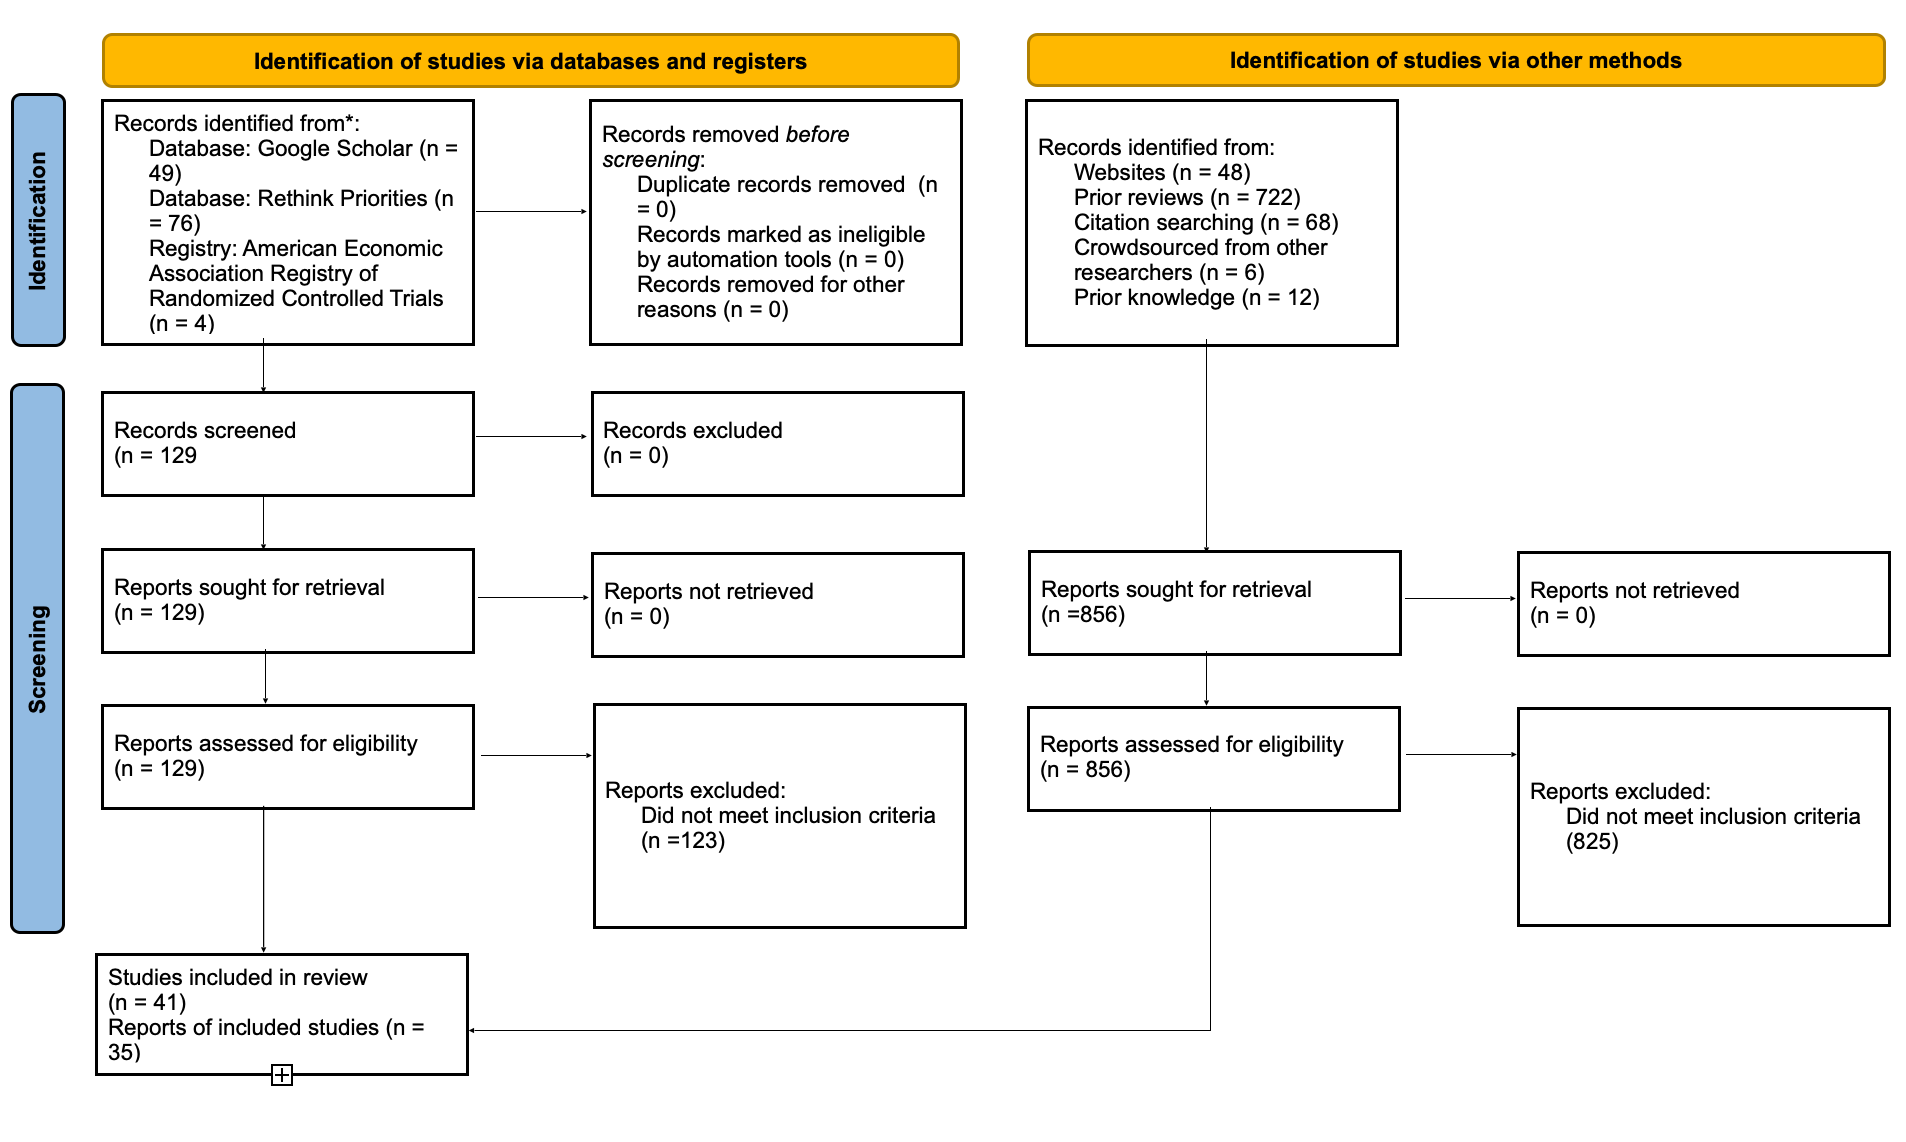
\includegraphics[width=1.2\linewidth,]{./figures/prisma-diagram} 

}

\caption{PRISMA diagram.}\label{fig:prisma_diagram}
\end{figure}

\subsection{Data extraction}\label{sec3.3}

The first author extracted all data. We extracted an effect size for one
outcome per intervention: the measure of net MAP or RPM consumption that
had the longest follow-up time after intervention. Additional variables
coded included information about publication, details of the
interventions, length of follow-ups, intervention theories, and
additional details about interventions' methods, contexts, and open
science practices (see accompanying code and data repository for full
documentation: \url{https://doi.org/10.24433/CO.6020578.v2}). When in
doubt about calculating effect sizes, we consulted publicly available
datasets and/or contacted authors. To assess risk of bias, we collected
data on whether outcomes were self-reported or objectively measured,
publication status, and presence of a pre-analysis plan and/or open data
(Supplement).

All effect size conversions were conducted by the first author using
methods and R code initially developed for previous papers
\citep{paluck2019, paluck2021, porat2024} using standard techniques
\citep{cooper2019}, with the exception of a difference in proportion
estimator that treats discrete events as draws from a Bernoulli
distribution (see appendix to \citep{paluck2021} for details). As our
measure of standardized mean difference, we used Glass's \(\Delta\)
whenever possible, defined as
\(\Delta = \frac{\mu_T - \mu_C}{\sigma_C}\), where \(\mu_T\) and
\(\mu_C\) respectively denote the treatment and control group means and
\(\sigma_C\) denotes the pre-treatment control group standard deviation.
If the control group SD was not available, we standardized on the pooled
SD. When means and SDs were not available, we converted effect sizes
from: regression coefficients, eta squared, or z-scores. When there was
insufficient information to calculate a specific SMD, but the text
reports the result as a null, we recorded the outcome as an
``unspecified null'' and set it to 0.01.

\subsection{Statistical analysis}\label{sec3.4}

We used \texttt{Rmarkdown} \citep{xie2018} and a containerized online
platform \citep{moreau2023, clyburne2019} to ensure computational
reproducibility \citep{polanin2020}. We conducted meta-analysis using
robust variance estimation (RVE) methods \citep{hedges2010} as
implemented by the \texttt{robumeta} package in \texttt{R}
\citep{fisher2015, Rlang}. Many studies in our sample compared multiple
treatment groups to a single control group. Therefore, we used the RVE
method to allow for the resulting dependence between observations, as
well as a standard small-sample correction.

Data analyses were largely conducted with custom functions building on
\texttt{tidyverse} \citep{wickham2019}. We assessed publication bias
using selection model methods \citep{hedges1992, vevea1995}, sensitivity
analysis methods \citep{mathur2024}, and the significance funnel plot
\citep{mathur2020}. These methods assume that the publication process
favors ``statistically significant'' (i.e., p \textless{} 0.05) and
positive results over ``nonsignificant'' or negative results. Our
sensitivity check meta-analyzes only non-affirmative results, which
creates an estimate under a hypothetical ``worst-case'' publication bias
scenario where affirmative studies are almost infinitely more likely to
be published than non-affirmative studies. We conducted these analyses
using functions in \texttt{metafor} \citep{viechtbauer2010} and
\texttt{PublicationBias} \citep{mathur2020, mathur2024}.

\section{Discussion}\label{discussion}

Our meta-analysis of RCTs estimated a small overall effect of SMD =
0.07, along with its upper confidence bound of SMD = 0.12. Effects were
also consistently small across an array of locations, study designs, and
intervention categories. Some individual studies found comparatively
larger effects ( e.g.~five studies estimated SMD \textgreater{} 0.5:
\citep{carfora2023, merrill2009, kanchanachitra2020, bianchi2022, piester2020}).
We view these these interventions as intriguing candidates for
subsequent research and replication, but their heterogeneous theories,
methods, and implementation details suggest that no singular approach,
means of delivery, or message should be considered a well-validated
method of reducing MAP consumption. Taken together, these findings
suggest that reducing MAP consumption is an unsolved problem.

Perhaps surprisingly, our results diverged from the more positive
findings of previous reviews
\citep{mathur2021meta, meier2022, mertens2022}, which are summarized in
the Supplement. Our much smaller estimate likely reflects our stricter
methodological inclusion criteria. For instance, of the ten largest
effect sizes in a previous meta-analysis
\citep{mathur2021effectiveness}, nine measured attitudes and/or
intentions, and the tenth came from a non-randomized design. Prior
research has found that intentions often do not predict behavior
\citep{mathur2021effectiveness}, and reviews in other fields have found
systematic differences in impacts between randomized and non-randomized
evaluations \citep{porat2024, stevenson2023}. Supporting this
interpretation, robustness checks in which we relaxed our methodological
inclusion criteria produced results similar to those of previous
reviews. This possibility will need further empirical evaluation.

Another potentially surprising result is that only two choice
architecture papers met our methodological inclusion criteria. Most
potentially eligible papers either measured hypothetical outcomes or
measured outcomes immediately after the intervention. Moreover, prior
reviews that found choice architecture approaches to be consistently
effective at modifying diet typically focused on foods that may have
weaker cultural and social attachments than MAP, such as sugary drinks
and snacks \citep{venema2020, adriaanse2009}. We speculate that changes
to how MAP is sold and consumed, by contrast, are more likely to be
noticed and to engender political and cultural backlash
\citep{popper2019}.

Likewise, as our analyses show, studies aimed at reducing RPM
consumption are associated with a considerably larger effect (SMD =
0.25) than those aimed at reducing all MAP consumption. In our search
for literature, we found that many prior reviews grouped MAP and RPM
studies together, treating their outcomes as aimed at a single
theoretical target \citep{slough2023}. However, if reductions in RPM
lead to consumers' substituting to other forms of MAP, then analyses
that synthesize the two categories of outcome may produce inflated
estimates of MAP reduction. We view such substitutions as likely: many
health guidelines, such as the heart-healthy diet \citep{diab2023},
encourage reducing RPM while also encourage moderate intake of poultry
and fish, both of which come with severe externalities, such as risking
zoonotic outbreaks from factory farms \citep{hafez2020} and causing land
and water pollution \citep{grvzinic2023}. Additionally, raising chicken
and fish may lead to substantially worse outcomes for animal welfare
\citep{mathur2022ethical}. Finally, newspaper articles and op-ed
frequently cite reducing RPM consumption as something consumers can and
should do to fight climate change \citep{moskin2022, carroll2019}. By
contrast, vegetarianism is still a minority diet worldwide
\citep{tilman2014} that consumers consider to be difficult,
unsatisfying, and expensive \citep{bryant2019}. We speculate that
cutting back on RPM may be perceived as easier and more socially
normative than is cutting back on all MAP. This possibility might
explain the observed difference in effect sizes.

Our analyses have limitations. Relatively few studies met our
methodological inclusion criteria, limiting statistical precision.
Additionally, as with all meta-regression analyses, ours should not be
interepreted as causal effects. That is, estimated differences in effect
sizes between groups of studies do not represent the causal effects of
the study characteristics (e.g., theoretical approach) on their
interventions' effects because studies' characteristics are not randomly
assigned. Finally, although our methodological inclusion criteria were
more stringent than those of previous reviews, the included studies
still had limitations. For example, many outcome measures in our
database were coarse, such as self-reports of whether participants ate
more or less MAP after treatment than than they typically did
\citep{aberman2018} without further quantification. Other studies
actively seek to associate eating MAP with a sense of threat
\citep{fehrenbach2015} or with endorsing social hierarchy
\citep{allen2002} and then collect self-reported outcomes. These designs
raise the possibility of social desirability bias.

Overall, this literature shows encouraging trends in methodology. First,
as noted, a majority of studies in our meta-analysis have been published
since 2020, indicating the field's increasing attention to rigorous
design and measurement. Second, we observe many fruitful collaborations
between researchers and advocacy organizations, as shown by the large
number of nonprofit white papers in our sample. Third, many promising
designs and interventions still await rigorous evaluation. For instance,
no study that met our criteria evaluated extended contact with farm
animals \citep{cerrato2022}, manipulations to the price of meat
\citep{wilde2016}, activating moral and/or physical disgust
\citep{palomo2018}, watching popular media such as the \emph{Simpsons}
episode ``Lisa the Vegetarian'' \citep{byrd2010} or the movie
\emph{Babe} \citep{novatna2019}, and many categories of choice
architecture intervention \citep{olafsson2024}. Moreover, emerging
research designs help address longstanding measurement challenges, such
as the possibility that interventions implemented at one time point
(e.g., choice architecture at a lunch buffet) create later compensatory
behavior (e.g., eating more MAP at dinner) \citep{vocski2024}.
Ultimately, our findings suggest that meaningfully reducing MAP
consumption is an unsolved problem, and points to the critical
importance of the field's increasing focus on methodological rigor.

\bmhead{Acknowledgments}

\emph{Thanks to Alex Berke, Alix Winter, Anson Berns, Dan Waldinger,
Hari Dandapani, Adin Richards, Martin Gould, Matt Lerner, Rye Geselowitz
and Sungwon Ma for comments on an early draft. Thanks to Jacob Peacock,
Andrew Jalil, Gregg Sparkman, Joshua Tasoff, Lucius Caviola, Natalia
Lawrence, and Emma Garnett for help with assembling the database and
providing guidance on their studies. Thanks to Sofia Vera Verduzco for
research assistance. We gratefully acknowledge funding from the NIH
(grant R01LM013866), Open Philanthropy, and the Food Systems Research
Fund (Grant FSR 2023-11-07).}

\section*{Declarations}\label{declarations}
\addcontentsline{toc}{section}{Declarations}

The authors declare no conflicts of interest. \newpage

\renewcommand\refname{References}
\bibliography{./vegan-refs.bib}


\end{document}
